%\documentclass[notes,10pt,aspectratio=169]{beamer}

\documentclass[10pt,aspectratio=169]{beamer}

%\usetheme{Singapore} %Boadilla, Madrid, default, etc. 
\usetheme[progressbar=frametitle]{metropolis}
\usecolortheme{rose} %beaver, dolphin, crane, 




\usecolortheme{default}

\usepackage[utf8]{inputenc}
\usepackage[T1]{fontenc}
\usepackage{lmodern}
\usepackage{xcolor}
\usepackage{tikz}
\usetikzlibrary{shapes.geometric, arrows, positioning}

\tikzstyle{block} = [rectangle, draw, text width=4cm, align=center, rounded corners, minimum height=1cm]
\tikzstyle{decision} = [rectangle, draw, text width=5cm, align=center, fill=blue!10, rounded corners, minimum height=1cm]
\tikzstyle{terminal} = [rectangle, draw, text width=4.5cm, align=center, fill=yellow!30, rounded corners, minimum height=1cm]
\tikzstyle{end} = [rectangle, draw, text width=5cm, align=center, fill=green!30, rounded corners, minimum height=1cm]
\tikzstyle{arrow} = [->, thick]




%2. change the bullets 
\setbeamertemplate{itemize item}[triangle] %circle, square,... 


% 1. Define custom colors and set colors 
%\definecolor{myblue}{HTML}{003366}
\definecolor{accent}{RGB}{78,205,196}

%\setbeamercolor{title}{fg=white,bg=myblue}
\setbeamercolor{frametitle}{fg=black,bg=white}
%\setbeamercolor{normal text}{fg=mygray}
\setbeamercolor{block title}{fg=black,bg=blue}
%\setbeamercolor{block body}{fg=black,bg=white}

\setbeamercolor{item}{fg= orange!80} % Change bullet color
\setbeamercolor{button}{bg=orange, fg=white}





% 3. BibLaTeX settings
\usepackage[
  backend=biber,
  style=apa,
  citestyle=authoryear
]{biblatex}
\addbibresource{references.bib}

\title{Centralized Annuities System}
%\subtitle{A Mini Literature Overview}

\author{%
 Lucas Condeza
\inst{1} \and
   %\and
%  Coauthor Three\inst{3}
}
\institute{
  \inst{1} Yale University \\
}

\date{\today}

\begin{document}

\begin{frame}
  \titlepage
\end{frame}


%%%%%%%%%%%%%%%%%%%%%%%
\begin{frame}{Pensions in Chile}    
    \begin{itemize}%[<+->]
        \item Workers save 10\% of their wage in a savings account 

        \begin{itemize}
            \item Similar to 401(k)
        \end{itemize} 
        
        \item Options when retiring: 
        \begin{itemize}
            \item \textit{Phased withdrawals} (AFP): overlife risk

            \item Annuity (insurers): 
        \end{itemize}
         \begin{align*}
     S = \mathbb{E}_{T} \left[\sum_{t=1}^T\frac{F}{(1+r)^t}| x_i\right]
 \end{align*}
 $S$: stock of savings, $F$: per period annuity payment, $x_i$: individual mortality factors
\end{itemize} 
\end{frame}


%%%%%%%%%%%%%%%%%%%%%%%%%

\begin{frame}{SCOMP} 
    \begin{itemize}%[<+->]
    \item SCOMP steps: 
    \begin{enumerate}
        \item Request of balance statement 
        \item Request for offers: asks for certain type of contracts (e.g. annuity)
        \item Insurers make offers (e.g. \$1000 per month)
        \item Retiree chooses one of the offers or asks for external offers

    \end{enumerate}

        \item External offers: bargaining and information disclosure
        %When offering insurers know 1. age, 2. amount of savings, 3. gender, 4. dependents. With external offers they learn your RUT(SSN): more information  
    

    \item Firms competition 1. financing cost 2. prediction algorithm 

    \begin{align*}
    \pi_{ji}(F) = S_i-  \mathbb{E}^j_{T} \left[\sum_{t=1}^T\frac{F}{(1+r_j)^t}|x_i \right]
    \end{align*}
    % if it was only financing cost, it would be a monopoly
    \end{itemize}
\end{frame}

%%%%%%%%%%%%%%%%%%%%%

 \begin{frame}{Data}
\begin{itemize}
    \item SCOMP data at the individual level  
    \begin{itemize}
        \item Offers received and accepted 
        \item Total savings 
        \item Demographics: age and gender
    \end{itemize}
     \item Retirement insurance companies: risk ratings, \#  of intermediaries and their  locations.
\end{itemize}


\end{frame}

%%%%%%%%%%%%%%%%%%


\begin{frame}{Research question: gov. guarantee}
\begin{itemize}
    \item Annuities puzzle: people \textit{should} buy annuities, in the US only 12\% do (\cite{modigliani_life_1986})

    \item Annuities: eliminate overlife risk, create insurer risk (Thaler et al. 2011) % insurer risk is not insurable. 

    \item Estimate valuation for eliminating insurer risk
    \begin{itemize}
        \item Unique data with individual's choice set 
        % to estimate demand one needs the choice set of individuals (in the case of cars this is trivial) but insurance is personalized, hence our data allows us to estimate demand which  one normally estimates demand by having the individual's choice set allows us to evaluate the 
        \item Identification sources: variation in 1) insurer risk variation and 2) existing gov. guarantee.  
\end{itemize}

\begin{figure}
    \centering
    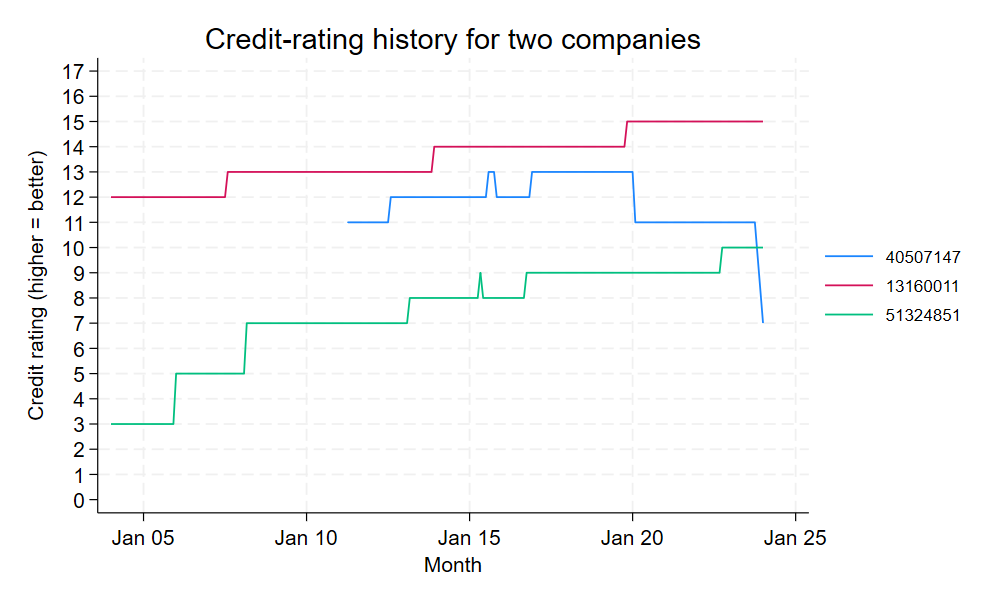
\includegraphics[width=0.5\linewidth]{../figures/credit_history.png}
    %\caption{Enter Caption}
    \label{fig:enter-label}
\end{figure}

  \end{itemize}
 
\end{frame}

\begin{frame}{Question 1: external offers}

\begin{itemize}
   
    \item 80\% of the signings are external offers. 
    \item What is the impact of allowing external offers? 

    \begin{itemize}
        \item Distributional consequences: pooling to separating equilibria - based on information disclosed in between

        % without the external offers they are pooled into one market based on first stage observables, whereas with the aftermarket they are separated based 

        \item Bargaining increases welfare vis a vis a price setting monopolists. What happens when there is competition? 
\end{itemize}   
\end{itemize}
\end{frame}

\begin{frame}{Model}

\begin{itemize}
    \item Individual $i$, of type $k$,  valuation for offer of insurer $j$: 

    $$ u_{ijt} = \beta X_{jt}+ \alpha_{k(i)} r_{ij} + \xi_j +\xi_{jt} + \varepsilon_{ijt}  $$

    where $r_{ij}$ is the interest rate, $X_{jt}$  are insurer characteristics (credit-rating, number of customer service offices), $\xi_j$ are persistent unobserved insurer characteristics, $\xi_{jt}$ mean-zero demand shocks.  

    The types are defined as combinations of age, gender and amount saved.

    \item Estimation by ML: 
    \begin{enumerate}
        \item Estimate  ($\delta_{jt}, \alpha_k$) to maximize the likelihood 
        \item Use $\mathbb{E}[\delta_{jt}|x_{jt},x_{-jt}]= 0$ to estimate ($\beta, \xi_j, \xi_{jt}$)
    \end{enumerate}
\end{itemize}
\end{frame}

\begin{frame}{Question 1 }
    \begin{itemize}
    \item Use estimated demand to estimate the increase in consumer welfare of exogenously increasing the credit rating of insurers 
    \item Allows to answer: 
    \begin{enumerate}
        \item Whether insurer risk explains a share of the annuities puzzle. By comparing the initial share of individuals buying annuities and the simulated share with higher credit ratings
        
        \item  Provides 
    \end{enumerate}
    \end{itemize}
        
\end{frame}


 

\end{document}